\chapter{RDF}
\label{chap:rdf}
Die bisherigen Kapitel bieten einen Überblick über die verschiedenen Methoden und Herangehensweisen des Knowledge Engineerings. Auch die wichtigsten theoretischen Grundlagen wurden mit den vorigen Kapiteln abgedeckt. Im Kapitel~\nameref{chap:ontologien} wurde gezeigt, dass für die Darstellung von Ontologien verschiedene Sprachen entwickelt wurden. In Diesem Beispiel wird eine der bekanntesten Ontologie-Sprachen, OWL (Web Ontology Language), verwendet. OWL basiert auf der Syntax von RDF.\ Folglich scheint es uns wichtig diese zwei Sprachen kurz vorzustellen.

Dieses Kapitel basiert auf der Spezifikation des W3C~\cite{w3rdf}.

Das "`Resource Description Framework"' (RDF) ist ein Framework um Informationen aus Ressourcen zu formulieren. Ressourcen können dabei Dokumente, Leute, Objekte aber auch abstrakter Inhalt sein. Mit RDF können Informationen im Web durch Anwendungen verarbeitet werden, anstatt diese nur anzuzeigen. RDF bietet ein gemeinsames Framework um die Informationen zwischen Anwendungen auszutauschen ohne die Bedeutung der Informationen zu verändern.

RDF ist die Grundlage des Sematic Web, welches die Flexibilität von RDF vollumfänglich ausnutzt. Alle Daten im Semantic Web werden in RDF abgebildet, wobei es RDF ermöglicht Daten zu verknüpfen. Dies führt dazu, dass zu einer Ressource mehr Informationen zusammen getragen werden.\cite{cambSemRDF}

\section{RDF Data Model}
\label{sec:rdf_rdf_dataModel}
Informationen werden in RDF als Aussagen abgebildet. Der Aufbau dieser ist immer gleich und weist die folgende Struktur eines Tripels auf:

\lstset{caption={Tripel-Struktur einer RDF-Aussage},captionpos=b}
\begin{lstlisting}
    <Subjekt> <Prädikat> <Objekt>
\end{lstlisting}

Eine RDF Aussage bildet eine Beziehung zwischen zwei Ressourcen (Entitäten), nämlich Subjekt und Objekt, ab. Das Prädikat repräsentiert die Beziehung zwischen den zwei Ressourcen. Die Beziehung wird in RDF als Eigenschaft (Property) abgebildet.
 
\noindent\hspace*{15mm} <Eine Programmiersprache> <hat> <ein Programmierparadigma>
\lstset{caption={Beispiel einer RDF-Aussage},captionpos=b}
\begin{lstlisting}
    <Seilpark> <hatStandort> <Balmberg>
\end{lstlisting}

Eine Entität kann in mehreren Tripeln referenziert werden. Es ist zudem möglich eine Ressource in einer Aussage als Objekt, in einer anderen Aussage aber als Subjekt zu verwenden. Dies ermöglicht es, Verbindungen zwischen mehreren Tripeln herzustellen. Dies ist ein wichtiger Teil von RDF.

\newpage

Tripel werden in sogenannte RDF-Graphen abgebildet. Diese bestehen aus Knoten und Pfeilen. Die Subjekte und die Objekte werden als Knoten, die Prädikate als Pfeile dargestellt. Genaueres dazu findet sich im Kapitel~\nameref{chap:graph_data}.

\begin{figure}[H]
\centering \rotatebox{0}{\scalebox{0.3}[0.3]{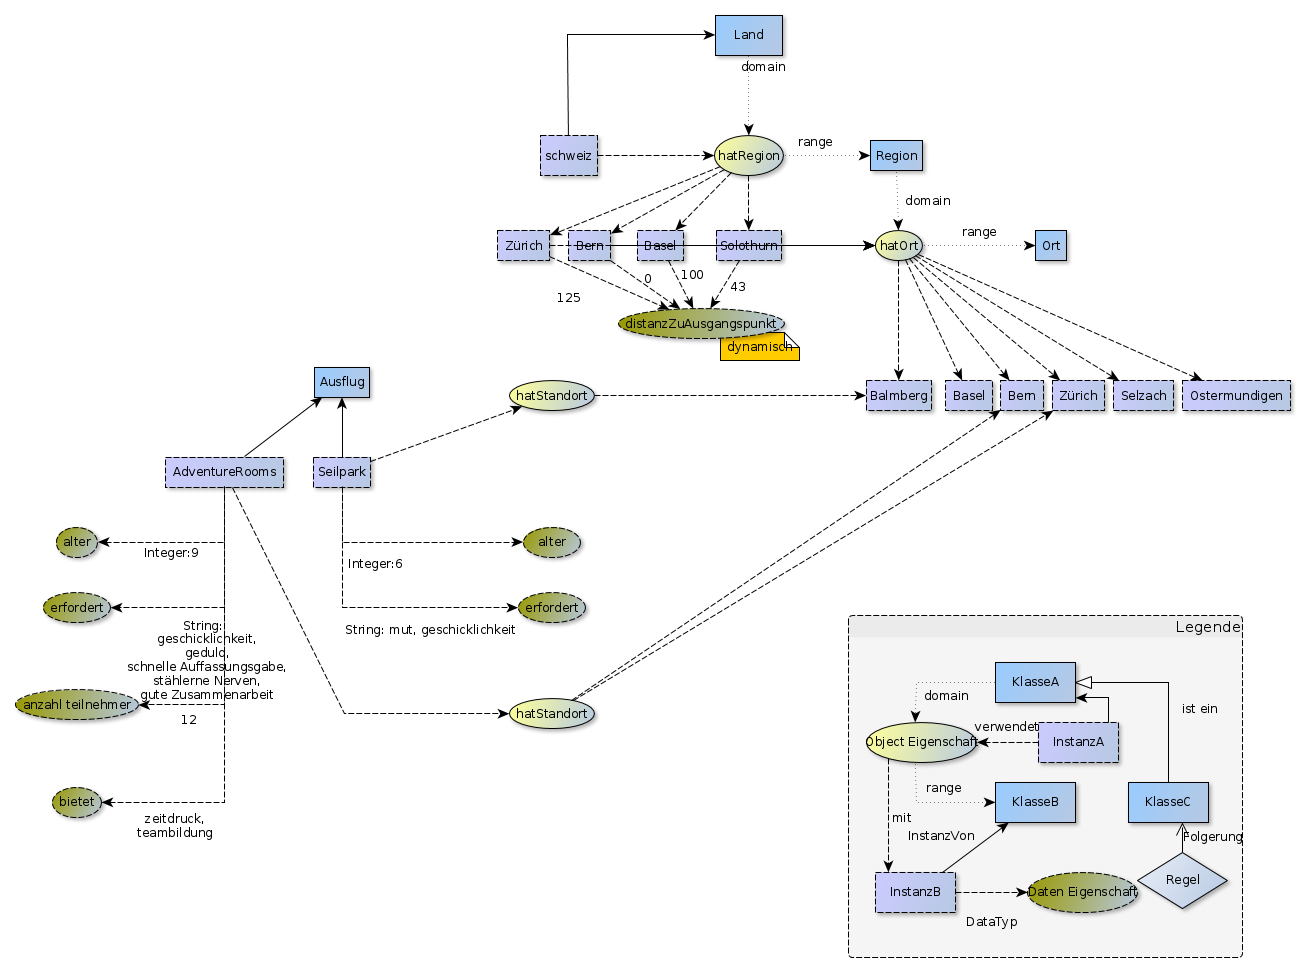
\includegraphics{bilder/rdf_reiseplaner_ontologie.png}}}
\caption{Ausschnitt der Ontologie des Reisplaners\label{fig:rdf_reiseplaner_ontologie}\protect\footnotemark}
\end{figure}
\footnotetext{Eigene Darstellung mittels yEd.}

Es gibt drei Typen von RDF-Daten, welche in Tripeln auftreten: Ressource-Knoten (IRIs), Literale und leere Knoten (Blank).

\subsection{IRIs (International Resource Identifier)}
\label{sec:rdf_rdf_dataModel_iris}
Wie der Name schon sagt, stellt ein IRI eine Ressource dar. Dabei handelt es sich um einen globalen Identifier, IRIS können also von verschiedenen Nutzern wiederverwendet werden. Es gibt verschieden Formen von IRIs, so zum Beispiel die URLs welche als Web-Adresse verwendet werden. Eine Andere Form der IRI bietet eine Kennung für eine Ressource ohne den Standort oder den Zugriff preiszugeben. Die genaue Spezifikation von IRIs findet sich unter \href{http://www.ietf.org/rfc/rfc3987.txt}{RFC 3987}.

IRIs können in allen drei Positionen eines Tripels auftreten.

\subsection{Literale Knoten}
\label{sec:rdf_rdf_dataModel_literal}
Der Begriff Literal wird als Synonym für Wert verwendet. Es handelt sich bei Literalen also um Basiswerte, die nicht IRIS sind. Literale können Strings, Datumswerte oder auch Nummern sein. Um die Werte richtig zu interpretieren, haben Literale einen Datentyp zugeordnet. Einem String kann zusätzlich eine Sprache zugewiesen werden.

Literale können in einem Tripel nur als Objekt verwendet werden.

\subsection{Leere Knoten (blank nodes)}
\label{sec:rdf_rdf_dataModel_blankNodes}
Ein leerer Knoten stellt eine Ressource ohne URI dar. Der Vorteil dieser Knoten ist, dass er keinen globalen Identifier braucht. Leere Knoten können mit einer einfachen Variable in der Algebra verglichen werden. Sie bilden ein Objekt ab, wobei der Wert zweitrangig ist.

Leere Knoten können in einem Tripel Subjekt oder Objekt sein.


\section{Multiple Graphs}
\label{sec:owlRdf_rdf_dataModel_multipleGraphs}
Eine der neuesten Erweiterung von RDF sind multipe Graphen. Diese wurden eingeführt um Teilmengen einer Tripelsammlungen zu definieren. Dieser Mechanismus stammt ursprünglich von der Abfragesprache SPARQL (siehe~\ref{chap:sparql}~\nameref{chap:sparql}). Man unterscheidet dabei ziwschen benannten (named) und unbenannten (unnamed) Graphen. Bei einem unbenannten Graphen enthalten die Tripel jeweils die gesamte URI.\@

\begin{lstlisting}[caption={Beispiel eines unbenannten (unnamed) Graphen}]
	<http://example.org/bob> <is published by> <http://example.org>.
\end{lstlisting}

Bei benannten Graphen wird ein Identifikator (identifier) geschaffen, auf welchen referenziert wird.

\begin{lstlisting}[caption={Beispiel eines benannten (named) Graphne}]
Identifier: 
		http://example.org/bob
Graph:
		<Bob> <is a> <person>.
		<Bob> <is a friend of> <Alice>.
\end{lstlisting}

Multipe Graphen eines RDF-Dokuments stellen eine Datenmenge dar. Sie bestehen standartmässig aus einem unbenannten (unnamed) Graphen, welcher der Basisgraph (default) ist, und mehreren benannten (named) Graphen.

\section{RDF Vokabular}
\label{sec:rdf_rdf_voca}
RDF wird typischerweise in Kombination mit Vokabular und Konventionen verwendet, welche semantische Daten als Ressourcen zur Verfügung stellen.

Um das Vokabular von RDF zu zu definieren, wird die RDF-Schema-Sprache unterstützt. Diese ermöglicht semantische Eigenschaften der RDF Daten zu definieren. Es kann damit festgelegt werden, welche Ressourcen an welcher Position verwendet werden.

So verwendet RDF zum Beispiel die Bezeichnung der Klasse um Ressourcen zu kategorisieren. Die Beziehungen zwischen Instanzen werden in Eigenschaften (properties) abgebildet. Mit RDF können auch Hierarchien im Bereich der Klassen, aber auch der Eigenschaften gebildet werden. Ausserdem können auf Objekten und Subjekten Typeinschränkungen vorgenommen werden.~\footnote{http://www.w3.org/TR/2014/NOTE-rdf11-primer-20140624/\#section-rdfa~\cite{w3rdf}}

\section{RDF Formen}
\label{sec:rdf_rdf_formen}
Es gibt verschiedene Formen um RDF niederzuschreiben. Diese führen schlussendlich alle zu denselben Tripeln, sie haben jedoch unterschiedliche Einsatzgebiete. So gibt es zum Beispiel die N-Tripel- oder die Turtle-Schreibweise. Im folgenden Kapitel soll aber die XML/RDF-Schreibweise kurz vorgestellt werden, da wir es in unserem Beispiel verwenden.

\subsection{XML/RDF}
\label{sec:rdf_rdf_formen_xmlRdf}
Bei XML/RDF handelt es sich um eine Schreibweise von RDF, welche die XML-Syntax verwendet um  RDF-Graphen abzubilden. Als RDF in den 1990er Jahren entwickelt wurde, war dies die einzige Schreibweise dafür.

In RDF/XML sind Tripel in einem XML Element \textit{rdf:RDF} spezifizert.  Das Element \textit{rdf:description} wird verwendet, um ein Tripel zu definieren, welches als Subjekt die im \textit{about}-Attribut definierte IRI Spezifikation hat. Ein Description-Element kann Unterelemente beinhalten. Der Name des Subelements is ein IRI, welches in der Eigenschaft \textit{rdf:type} abgebildet ist. Dabei repräsentiert jedes Subelement ein Tripel. Handelt es sich beim Objekt eines Tripels auch um ein IRI, hat das Unterelement keinen Inhalt. Der Objekt-IRI-Knoten wird durch ein \textit{rdf:resource}-Attribut beschrieben.

Wenn das Objekt eines Tripels ein Literal ist, wird der Literalwert als Inhalt des Elements angegeben. Datentypen werden auch als Attribute eines Elementes angegeben.

\begin{lstlisting}[caption={Beispiel RDF Elemente\protect\footnotemark}]
<!DOCTYPE rdf:RDF [
    <!ENTITY owl "http://www.w3.org/2002/07/owl#" >
    <!ENTITY swrl "http://www.w3.org/2003/11/swrl#" >
    <!ENTITY swrlb "http://www.w3.org/2003/11/swrlb#" >
    <!ENTITY xsd "http://www.w3.org/2001/XMLSchema#" >
    <!ENTITY rdfs "http://www.w3.org/2000/01/rdf-schema#" >
    <!ENTITY rdf "http://www.w3.org/1999/02/22-rdf-syntax-ns#" >
]>


<rdf:RDF xmlns="http://www.semanticweb.org/mira/ontologies/2014/9/FamilyOnto#"
     xml:base="http://www.semanticweb.org/mira/ontologies/2014/9/FamilyOnto"
     xmlns:rdfs="http://www.w3.org/2000/01/rdf-schema#"
     xmlns:swrl="http://www.w3.org/2003/11/swrl#"
     xmlns:owl="http://www.w3.org/2002/07/owl#"
     xmlns:xsd="http://www.w3.org/2001/XMLSchema#"
     xmlns:swrlb="http://www.w3.org/2003/11/swrlb#"
     xmlns:rdf="http://www.w3.org/1999/02/22-rdf-syntax-ns#">
    <owl:Ontology rdf:about="http://www.semanticweb.org/mira/ontologies/2014/9/FamilyOnto"/>
    <rdf:Description>
        <rdf:type rdf:resource="&swrl;IndividualPropertyAtom"/>
        <swrl:propertyPredicate rdf:resource="http://www.semanticweb.org/mira/ontologies/2014/9/FamilyOnto#isAncestor"/>
        <swrl:argument1 rdf:resource="urn:swrl#a"/>
        <swrl:argument2 rdf:resource="urn:swrl#x"/>
    </rdf:Description>
</rdf:RD>
\end{lstlisting}
\footnotetext{Eigenes Beispiel}
